\documentclass[12pt,landscape]{article}
\begin{document}



\subsection{Estimation Results of Regional Analysis}
First, simple linear regression models were fitted to the observations in each region, and 95\% confidence intervals for the education variable coefficients were returned to examine the overall pattern of regional diversity in education payoffs. A visual inspection of Figure \ref{fig:4.1} is illustrative of the fact that Russian regions are rather heterogeneous in terms of premiums to education. Following the basic Mincerian equation, we present the results of the multilevel regression.

\begin{figure}[htp]
	\begin{minipage}[b]{.5\linewidth}
		\centering
		\hspace*{-0.4in}
		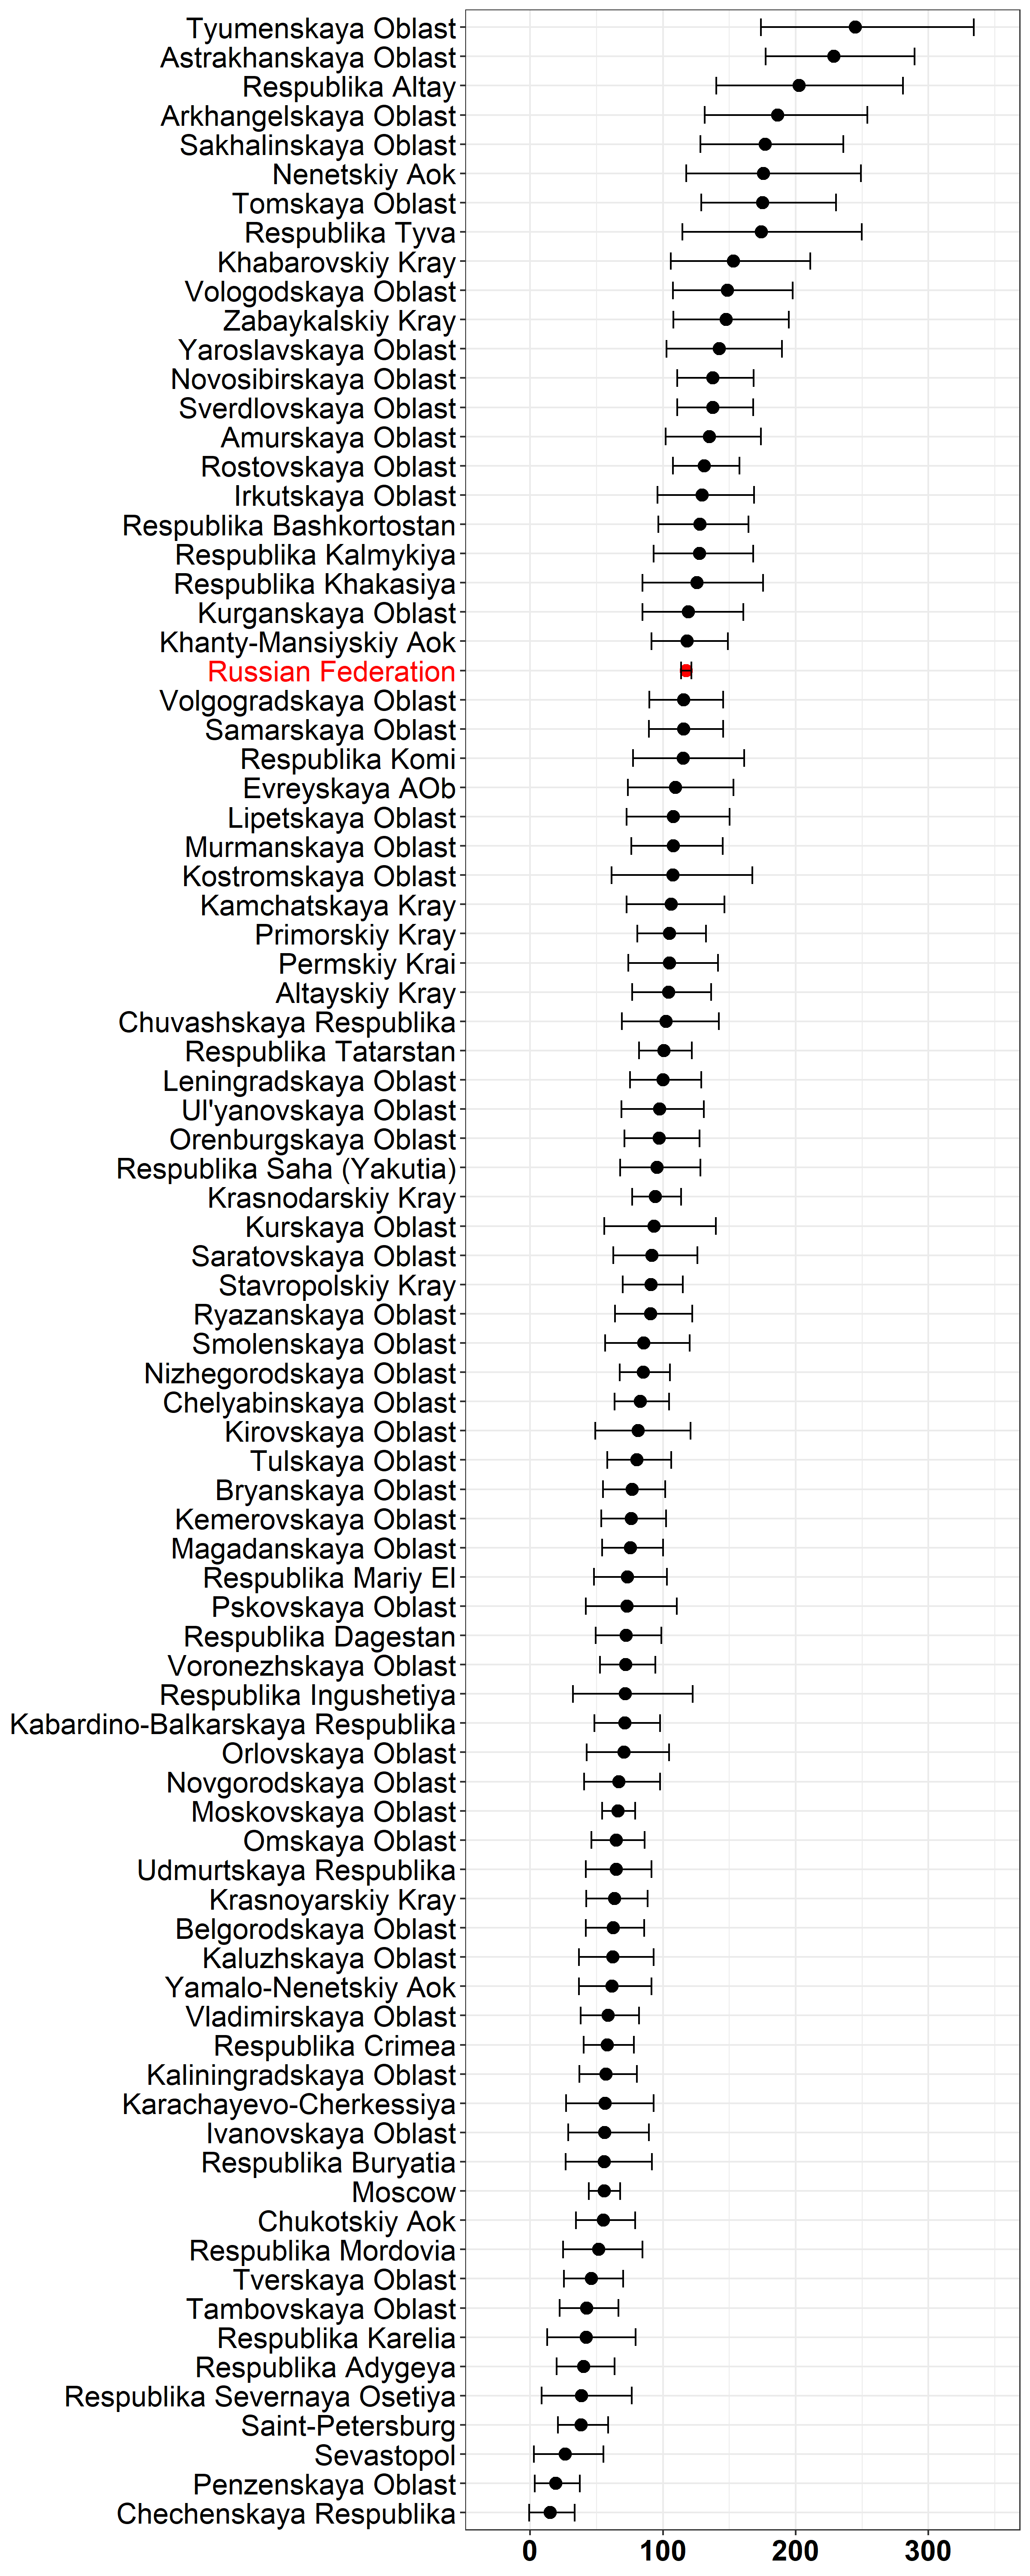
\includegraphics[width=250pt]{reg_he_18.png}
		% plot 1
		\subcaption{Higher Education}\label{}
	\end{minipage}
	\hfill
	\begin{minipage}[b]{.5\linewidth}
		\centering
		\hspace*{-0.2in}
		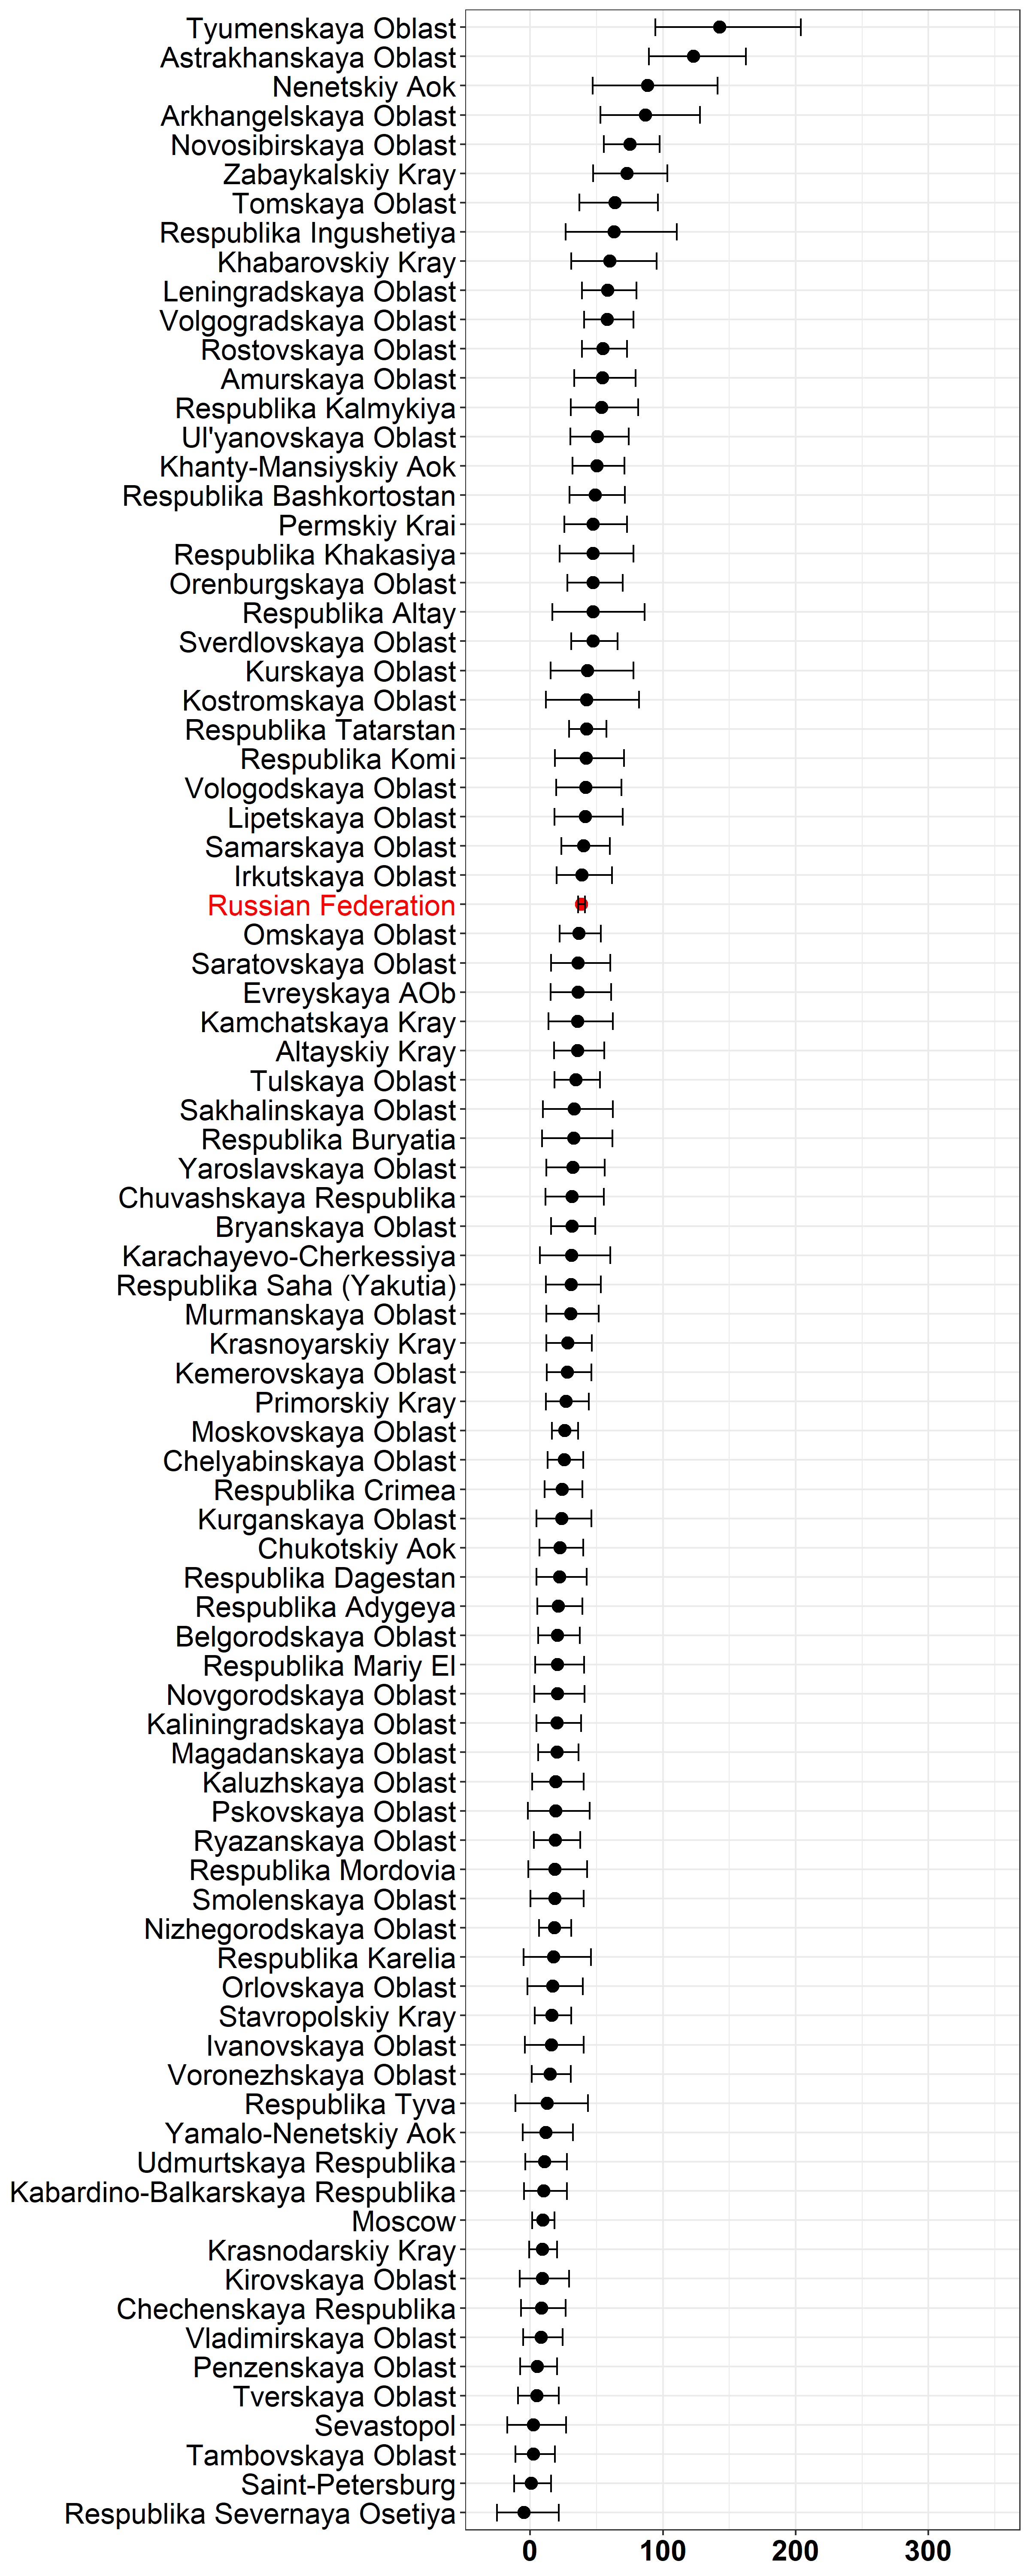
\includegraphics[width=250pt]{reg_ve_18.png}
		% plot 2
		\subcaption{Vocational Education}\label{}
	\end{minipage}
	\caption{Rates of Returns (Percentages) to Higher and Vocational Education in Russian Regions, Rosstat 2018}\label{fig:4.1}
\end{figure}

A two-level model without covariates was initially specified and indicated that the Intra-class Correlation (ICC) was equal to 16\%, i.e., 16\% of the variation in wage outcome was between regions. This is a high enough level to justify the estimation of a random effects model with covariates. Nested models comparison showed that there is a statistically significant regional variation in the effect of education on people's earnings ($-2\bigtriangleup LL(1) = 413.54, p < .001$).

Next, we examined the possible causes of this variation by adding the second-level independent variables and their interactions with education. The investigation revealed that none of the second-level characteristics are capable of changing the association between education and the amount of money Russians earn, except for \textit{the coverage by vocational education}. Substantively, it means that growth in the number of students covered by vocational programs leads to higher schooling premiums concerning both vocational and university education. As for the estimates obtained, sufficiently high vocational education coverage degree (when its standardized version is 1) corresponds to the average return rate of 30.6\%; medium vocational education coverage degree (when its standardized version is 0) corresponds to the average return rate of 35.8\%; low vocational education coverage degree (when its standardized version is -1) corresponds to the average return rate of 25.5\%. The interpretation of such a finding can imply that this quantity-related dimension of vocational education has the potential to serve as an instrument of boosting financial payoffs from post-secondary education in Russian regions. 


\printbibliography

\newpage
\section*{Appendix}
\addcontentsline{toc}{section}{Appendix}%

\setcounter{table}{0}
\renewcommand{\thetable}{A\arabic{table}}


\begin{table}[!htbp] \centering 
\caption{Results of Estimating Human Capital Depreciation for the Female sample, RLMS} 
	\label{tab:A1}
\begin{tabular}{@{\extracolsep{5pt}}lcccccc} 
\\[-1.8ex]\hline 
\hline \\[-1.8ex] 
& \textbf{1994} & \textbf{1998} & \textbf{2003} & \textbf{2006} & \textbf{2012} & \textbf{2018} \\ 
\\[-1.8ex] & (1) & (2) & (3) & (4) & (5) & (6)\\ 
\hline \\[-1.8ex] 
 Constant & 9.725$^{***}$ & 3.786$^{***}$ & 5.464$^{***}$ & 6.946$^{***}$ & 8.133$^{***}$ & 8.767$^{***}$ \\ 
  & (0.381) & (0.322) & (0.301) & (0.247) & (0.186) & (0.242) \\ 
  & & & & & & \\ 
 Educ, years ($S$) & 0.122$^{***}$ & 0.153$^{***}$ & 0.158$^{***}$ & 0.118$^{***}$ & 0.087$^{***}$ & 0.066$^{***}$ \\ 
  & (0.025) & (0.022) & (0.020) & (0.016) & (0.012) & (0.015) \\ 
  & & & & & & \\ 
 Educ X Exper ($TS$) & $-$0.002$^{*}$ & $-$0.002$^{***}$ & $-$0.002$^{**}$ & $-$0.0002 & $-$0.0001 & 0.0004 \\ 
  & (0.001) & (0.001) & (0.001) & (0.001) & (0.0005) & (0.001) \\ 
  & & & & & & \\ 
 Exper ($T$) & 0.074$^{***}$ & 0.080$^{***}$ & 0.055$^{***}$ & 0.013 & 0.020$^{**}$ & 0.020$^{*}$ \\ 
  & (0.019) & (0.016) & (0.015) & (0.013) & (0.010) & (0.011) \\ 
  & & & & & & \\ 
 Exper squared ($T^2$) & $-$0.001$^{***}$ & $-$0.001$^{***}$ & $-$0.001$^{***}$ & $-$0.0003$^{**}$ & $-$0.0005$^{***}$ & $-$0.001$^{***}$ \\ 
  & (0.0002) & (0.0002) & (0.0002) & (0.0001) & (0.0001) & (0.0001) \\ 
  & & & & & & \\ 
\hline \\[-1.8ex] 
Observations & 1,645 & 1,667 & 2,093 & 2,630 & 4,057 & 3,312 \\ 
R$^{2}$ & 0.051 & 0.089 & 0.110 & 0.139 & 0.104 & 0.092 \\ 
Adjusted R$^{2}$ & 0.049 & 0.087 & 0.108 & 0.138 & 0.103 & 0.091 \\ 
Residual Std. Error & 0.853 & 0.728 & 0.731 & 0.664 & 0.641 & 0.597 \\ 
F Statistic & 22.179$^{***}$ & 40.520$^{***}$ & 64.342$^{***}$ & 106.385$^{***}$ & 117.366$^{***}$ & 83.993$^{***}$ \\ 
\hline 
\hline \\[-1.8ex] 
\textit{Note:}  & \multicolumn{6}{r}{$^{*}$p$<$0.1; $^{**}$p$<$0.05; $^{***}$p$<$0.01} \\ 
\end{tabular} 
\end{table} 


\begin{table}[!htbp] \centering 
\caption{Results of Estimating Human Capital Depreciation for the Male sample, RLMS} 
	\label{tab:A2}
\begin{tabular}{@{\extracolsep{5pt}}lcccccc} 
\\[-1.8ex]\hline 
\hline \\[-1.8ex] 
& \textbf{1994} & \textbf{1998} & \textbf{2003} & \textbf{2006} & \textbf{2012} & \textbf{2018} \\ 
\\[-1.8ex] & (1) & (2) & (3) & (4) & (5) & (6)\\ 
\hline \\[-1.8ex] 
 Constant & 10.357$^{***}$ & 5.029$^{***}$ & 7.334$^{***}$ & 8.067$^{***}$ & 8.771$^{***}$ & 9.094$^{***}$ \\ 
  & (0.433) & (0.360) & (0.282) & (0.243) & (0.157) & (0.185) \\ 
  & & & & & & \\ 
 Educ, years ($S$) & 0.136$^{***}$ & 0.123$^{***}$ & 0.080$^{***}$ & 0.077$^{***}$ & 0.077$^{***}$ & 0.077$^{***}$ \\ 
  & (0.028) & (0.024) & (0.019) & (0.016) & (0.010) & (0.012) \\ 
  & & & & & & \\ 
 Educ X Exper ($TS$) & $-$0.002$^{*}$ & $-$0.001 & 0.0004 & $-$0.0003 & $-$0.0004 & $-$0.001 \\ 
  & (0.001) & (0.001) & (0.001) & (0.001) & (0.0005) & (0.001) \\ 
  & & & & & & \\ 
 Exper ($T$) & 0.054$^{**}$ & 0.032$^{*}$ & 0.002 & 0.007 & 0.035$^{***}$ & 0.037$^{***}$ \\ 
  & (0.023) & (0.017) & (0.014) & (0.013) & (0.009) & (0.010) \\ 
  & & & & & & \\ 
 Exper squared ($T^2$) & $-$0.001$^{***}$ & $-$0.0004$^{**}$ & $-$0.0003$^{*}$ & $-$0.0003$^{*}$ & $-$0.001$^{***}$ & $-$0.001$^{***}$ \\ 
  & (0.0003) & (0.0002) & (0.0002) & (0.0001) & (0.0001) & (0.0001) \\ 
  & & & & & & \\ 
\hline \\[-1.8ex] 
Observations & 1,392 & 1,433 & 1,763 & 2,170 & 3,360 & 2,800 \\ 
R$^{2}$ & 0.057 & 0.070 & 0.078 & 0.074 & 0.153 & 0.110 \\ 
Adjusted R$^{2}$ & 0.054 & 0.067 & 0.076 & 0.072 & 0.152 & 0.108 \\ 
Residual Std. Error & 0.951 & 0.803 & 0.754 & 0.688 & 0.598 & 0.570 \\ 
F Statistic & 20.989$^{***}$ & 26.879$^{***}$ & 37.362$^{***}$ & 43.281$^{***}$ & 151.868$^{***}$ & 86.125$^{***}$ \\ 
\hline 
\hline \\[-1.8ex] 
\textit{Note:}  & \multicolumn{6}{r}{$^{*}$p$<$0.1; $^{**}$p$<$0.05; $^{***}$p$<$0.01} \\ 
\end{tabular} 
\end{table} 



\begin{table}[!htbp] \centering 
	\caption{Results of Multilevel Modeling with Coverage by Vocational Education, Rosstat 2018} 
	\label{tab:A2} 
	\begin{tabular}{@{\extracolsep{5pt}}lcccc} 
		\\[-1.8ex]\hline 
		\hline \\[-1.8ex] 
		& Null model & Mincerian & Random Slope & Cross-Level Interaction \\ 
		\\[-1.8ex] & (1) & (2) & (3) & (4)\\ 
		\hline \\[-1.8ex] 
		Constant & 10.178$^{***}$ & 10.032$^{***}$ & 10.056$^{***}$ & 10.065$^{***}$ \\ 
		& (0.034) & (0.034) & (0.036) & (0.036) \\ 
		& & & & \\ 
		Vocational &  & 0.283$^{***}$ & 0.279$^{***}$ & 0.267$^{***}$ \\ 
		&  & (0.009) & (0.021) & (0.021) \\ 
		& & & & \\ 
		Higher &  & 0.638$^{***}$ & 0.641$^{***}$ & 0.622$^{***}$ \\ 
		&  & (0.009) & (0.025) & (0.025) \\ 
		& & & & \\ 
		Coverage VE X Vocational &  &  &  & 0.050$^{**}$ \\ 
		&  &  &  & (0.025) \\ 
		& & & & \\ 
		Coverage VE X Higher &  &  &  & 0.083$^{***}$ \\ 
		&  &  &  & (0.030) \\ 
		& & & & \\ 
		Experience &  & $-$0.026$^{***}$ & $-$0.027$^{***}$ & $-$0.027$^{***}$ \\ 
		&  & (0.002) & (0.002) & (0.002) \\ 
		& & & & \\ 
		Experience squared &  & $-$0.065$^{***}$ & $-$0.065$^{***}$ & $-$0.065$^{***}$ \\ 
		&  & (0.002) & (0.002) & (0.002) \\ 
		& & & & \\ 
		Females &  & $-$0.403$^{***}$ & $-$0.404$^{***}$ & $-$0.404$^{***}$ \\ 
		&  & (0.005) & (0.005) & (0.005) \\ 
		& & & & \\ 
		Coverage VE &  &  & $-$0.101$^{***}$ & $-$0.142$^{***}$ \\ 
		&  &  & (0.039) & (0.043) \\ 
		& & & & \\ 
		\hline
		\hline
		Variance of Intecept & 0.09 & 0.08 & 0.09 & 0.09 \\ 
		Variance of Vocational &  &  & 0.02 & 0.02 \\ 
		Variance of Higher &  &  & 0.04 & 0.04 \\ 
		Residual Deviance & 0.45 & 0.35 & 0.34 & 0.34 \\ 
		\hline
		\hline
		Observations & 49,187 & 49,187 & 49,187 & 49,187 \\ 
		Log Likelihood & $-$59,755.060 & $-$53,289.500 & $-$53,094.620 & $-$53,096.640 \\ 
		Akaike Inf. Crit. & 119,516.100 & 106,595.000 & 106,217.200 & 106,225.300 \\ 
		Bayesian Inf. Crit. & 119,542.500 & 106,665.400 & 106,340.500 & 106,366.100 \\ 
		\hline 
		\hline \\[-1.8ex] 
		\textit{Note:}  & \multicolumn{4}{r}{$^{*}$p$<$0.1; $^{**}$p$<$0.05; $^{***}$p$<$0.01} \\ 
	\end{tabular} 
\end{table} 




\end{document}
